%%%%%%%%%%%%%%%%%%%%%%%%%%%%%%%%%%%%%%%%%%%%%%%%%%%%%%%%%%%%%%%%%%%%%%%%%%%%%%%%
%% Plantilla de memoria en LaTeX para la ETSIT - Universidad Rey Juan Carlos
%%
%% Por Gregorio Robles <grex arroba gsyc.urjc.es>
%%     Grupo de Sistemas y Comunicaciones
%%     Escuela Técnica Superior de Ingenieros de Telecomunicación
%%     Universidad Rey Juan Carlos
%% (muchas ideas tomadas de Internet, colegas del GSyC, antiguos alumnos...
%%  etc. Muchas gracias a todos)
%%
%% La última versión de esta plantilla está siempre disponible en:
%%     https://github.com/gregoriorobles/plantilla-memoria
%%
%% Para obtener PDF, ejecuta en la shell:
%%   make
%% (las imágenes deben ir en PNG o JPG)

%%%%%%%%%%%%%%%%%%%%%%%%%%%%%%%%%%%%%%%%%%%%%%%%%%%%%%%%%%%%%%%%%%%%%%%%%%%%%%%%

\documentclass[a4paper, 12pt]{book}
%\usepackage[T1]{fontenc}

\usepackage[a4paper, left=2.5cm, right=2.5cm, top=3cm, bottom=3cm]{geometry}
\usepackage{times}
\usepackage[latin1]{inputenc}
\usepackage[spanish]{babel} % Comenta esta línea si tu memoria es en inglés
\usepackage{url}
%\usepackage[dvipdfm]{graphicx}
\usepackage{graphicx}
\usepackage{float}  %% H para posicionar figuras
\usepackage[nottoc, notlot, notlof, notindex]{tocbibind} %% Opciones de índice
\usepackage{latexsym}  %% Logo LaTeX
\usepackage{subfig}
\title{Memoria del Proyecto}
\author{Nombre del autor}
\usepackage[spanish]{babel}
\usepackage[latin1]{inputenc}
\usepackage{listings}
\renewcommand{\baselinestretch}{1.5}  %% Interlineado

\begin{document}

\renewcommand{\refname}{Bibliografía}  %% Renombrando
\renewcommand{\appendixname}{Apéndice}

%%%%%%%%%%%%%%%%%%%%%%%%%%%%%%%%%%%%%%%%%%%%%%%%%%%%%%%%%%%%%%%%%%%%%%%%%%%%%%%%
% PORTADA

\begin{titlepage}
\begin{center}
\begin{tabular}[c]{c c}
%\includegraphics[bb=0 0 194 352, scale=0.25]{logo} &
\includegraphics[scale=0.25]{img/logo_vect.png} &
\begin{tabular}[b]{l}
\Huge
\textsf{UNIVERSIDAD} \\
\Huge
\textsf{REY JUAN CARLOS} \\
\end{tabular}
\\
\end{tabular}

\vspace{3cm}

\Large
GRADO EN INGENIERÍA DE TELEMÁTICA

\vspace{0.4cm}

\large
Curso Académico 2015/2016

\vspace{0.8cm}

Trabajo Fin de Grado

\vspace{2.5cm}

\LARGE
BESTFORK\\
\small
APLICACIÓN WEB DE ANALISIS DE REPOSITORIOS GITHUB CON CÓDIGO PYTHON
\vspace{4cm}

\large
Autor : Iván López Barrio \\
Tutor : Dr. Gregorio Robles
\end{center}
\end{titlepage}

\newpage
\mbox{}
\thispagestyle{empty} % para que no se numere esta pagina


%%%%%%%%%%%%%%%%%%%%%%%%%%%%%%%%%%%%%%%%%%%%%%%%%%%%%%%%%%%%%%%%%%%%%%%%%%%%%%%%
%%%% Para firmar
\clearpage
\pagenumbering{gobble}
\chapter*{}

\vspace{-4cm}
\begin{center}
\LARGE
\textbf{Proyecto Fin de Carrera}

\vspace{1cm}
\large
Bestfork

\vspace{1cm}
\large
\textbf{Autor :} Iván López Barrio\\
\textbf{Tutor :} Dr. Gregorio Robles Martínez

\end{center}

\vspace{1cm}
La defensa del presente Proyecto Fin de Carrera se realizó el día \qquad$\;\,$ de \qquad\qquad\qquad\qquad \newline de 2016, siendo calificada por el siguiente tribunal:


\vspace{0.5cm}
\textbf{Presidente:}

\vspace{1.2cm}
\textbf{Secretario:}

\vspace{1.2cm}
\textbf{Vocal:}


\vspace{1.2cm}
y habiendo obtenido la siguiente calificación:

\vspace{1cm}
\textbf{Calificación:}


\vspace{1cm}
\begin{flushright}
Fuenlabrada, a \qquad$\;\,$ de \qquad\qquad\qquad\qquad de 2016
\end{flushright}

%%%%%%%%%%%%%%%%%%%%%%%%%%%%%%%%%%%%%%%%%%%%%%%%%%%%%%%%%%%%%%%%%%%%%%%%%%%%%%%%
%%%% Dedicatoria

\chapter*{}
\pagenumbering{Roman} % para comenzar la numeracion de paginas en numeros romanos
\begin{flushright}
\textit{Dedicado a \\
mis padres Martín, Rosalia y a mi hermana Leticia.\\
Os quiero.}
\end{flushright}

%%%%%%%%%%%%%%%%%%%%%%%%%%%%%%%%%%%%%%%%%%%%%%%%%%%%%%%%%%%%%%%%%%%%%%%%%%%%%%%%
%%%% Agradecimientos

\chapter*{Agradecimientos}
%\addcontentsline{toc}{chapter}{Agradecimientos} % si queremos que aparezca en el índice
\markboth{AGRADECIMIENTOS}{AGRADECIMIENTOS} % encabezado 

Quiero dar las gracias a mis padres, Martín y Rosalía. Por haber sido una motivación diaria para no rendirme y trabajar por lo que quería. Respetando siempre todas mis decisiones y confiando en mi. Estoy seguro de que sin ellos nada de esto hubiera sido posible  \\
Por supuesto, dar las gracias a mis amigos Yeray, Sergio, Alex, Justo, Helios, Arancha, Laura, Sandra, Estefania y Alberto, que en todos estos años me han sacado un montón de sonrisas.\\
No puedo olvidarme de Adrian y Kevin, con los que he compartido toda mi vida universitaria, pasando muchas horas juntos en los laboratorios y en la biblioteca, con muchos agobios, pero sabiendo que cualquier problema lo sacaríamos adelante.\\
Y mención especial a mi hermana Leticia, que se que siempre ha confiado en mi, que ha creido en mi incluso cuando ni siquiera yo creía, y que aunque ella no lo sabe, soy su mayor admirador. Te quiero.\\

Y muchas gracias a todos los que a lo largo de estos años, me han ayudado de una forma u otra.

%%%%%%%%%%%%%%%%%%%%%%%%%%%%%%%%%%%%%%%%%%%%%%%%%%%%%%%%%%%%%%%%%%%%%%%%%%%%%%%%
%%%% Resumen

\chapter*{Resumen}
%\addcontentsline{toc}{chapter}{Resumen} % si queremos que aparezca en el índice
\markboth{RESUMEN}{RESUMEN} % encabezado

Este proyecto es una Aplicación Web. La aplicación consiste en que, una vez proporcionada una URL de un repositorio GitHub por un usuario, la aplicación analizará el código escrito en Python del repositorio y sus Forks, otorgando una puntuación a cada uno de ellos en función de la calidad de código escrito. Luego le devolverá al usuario una página con los resultados ordenados de la mejor puntuación a la peor. Sus objetivos son: Ayudar a los desarrolladores a seleccionar de inicio el mejor código cuando se interesen en un repositorio; como dueño del repositorio, saber si la gente que trabaja en tu código está haciendo buenas mejoras; por último, servir como argumento al hacer un pull request.

Para realizar esta aplicación web, hemos empleado las últimas tecnologías web. En la parte del Servidor hemos utilizado: Django, Python, API de GitHub, Pylint y SQLite3, y para el cliente: HTML5, JavaScript, CSS3 y Bootstrap.

El proyecto, surge por la necesidad de crear una herramienta para aprovechar mejor el potencial de GitHub.


%%%%%%%%%%%%%%%%%%%%%%%%%%%%%%%%%%%%%%%%%%%%%%%%%%%%%%%%%%%%%%%%%%%%%%%%%%%%%%%%
%%%% Resumen en inglés

\chapter*{Summary}
%\addcontentsline{toc}{chapter}{Summary} % si queremos que aparezca en el índice
\markboth{SUMMARY}{SUMMARY} % encabezado

This project is a web application. The main objective is to analyze  Github repositories with Python code. The web aplication retrieves information about its forks and calculates the score depending on the code quality. Then it retuns a list of the forks of the repository sorted by this rating. The main objetives are: Help developers to choose the best fork to begin some project; if it is your own repository, you can know if other developers are doing a good job and, by last, it serves as an argument for a pull request.

For this project, we have used the last technologies on the server side, like as:  Django, Python, API de GitHub, Pylint y SQLite3,and for the client side, like as: HTML5, JavaScript, CSS3 y Bootstrap.

This project arises from the need to make an application that leverages the features of GitHub.
%%%%%%%%%%%%%%%%%%%%%%%%%%%%%%%%%%%%%%%%%%%%%%%%%%%%%%%%%%%%%%%%%%%%%%%%%%%%%%%%
%%%%%%%%%%%%%%%%%%%%%%%%%%%%%%%%%%%%%%%%%%%%%%%%%%%%%%%%%%%%%%%%%%%%%%%%%%%%%%%%
% ÍNDICES %
%%%%%%%%%%%%%%%%%%%%%%%%%%%%%%%%%%%%%%%%%%%%%%%%%%%%%%%%%%%%%%%%%%%%%%%%%%%%%%%%

% Las buenas noticias es que los índices se generan automáticamente.
% Lo único que tienes que hacer es elegir cuáles quieren que se generen,
% y comentar/descomentar esa instrucción de LaTeX.

%%%% Índice de contenidos
\tableofcontents 
%%%% Índice de figuras
\cleardoublepage
%\addcontentsline{toc}{chapter}{Lista de figuras} % para que aparezca en el indice de contenidos
\listoffigures % indice de figuras
%%%% Índice de tablas
%\cleardoublepage
%\addcontentsline{toc}{chapter}{Lista de tablas} % para que aparezca en el indice de contenidos
%\listoftables % indice de tablas


%%%%%%%%%%%%%%%%%%%%%%%%%%%%%%%%%%%%%%%%%%%%%%%%%%%%%%%%%%%%%%%%%%%%%%%%%%%%%%%%
%%%%%%%%%%%%%%%%%%%%%%%%%%%%%%%%%%%%%%%%%%%%%%%%%%%%%%%%%%%%%%%%%%%%%%%%%%%%%%%%
% INTRODUCCIÓN %
%%%%%%%%%%%%%%%%%%%%%%%%%%%%%%%%%%%%%%%%%%%%%%%%%%%%%%%%%%%%%%%%%%%%%%%%%%%%%%%%

\cleardoublepage
\chapter{Introducción}
\label{sec:intro} % etiqueta para poder referenciar luego en el texto con ~\ref{sec:intro}
\pagenumbering{arabic} % para empezar la numeración de página con números

Cuando los ordenadores empezaban a hacerse presente en la sociedad, nadie podía imaginarse la cantidad de personas que iban a dedicar su vida a trabajar con ellos y para ellos. Con la llegada de internet al hogar, se abría una puerta a mucha información. ¿Cómo ordenarla?, en el caso de la programación, hay múltiples lenguajes y diferentes tipos de programación.
La comunidad de Software libre, vio la necesidad de centralizar su trabajo y que todo el mundo tuviese acceso a esos trabajos. Es por ello que nació SourceForge en el año 1999. Trás el rápido éxito de SourceForge, grandes empresas como Google con ``Google Code'', o Atlassian con ``Bitbucket'' sacaron sus propios proyectos. A partir de la misma idea, en el año 2008, nacio GitHub que usaba Git para gestionar los proyectos y hacerlos colaborativos.

Pero hoy en día, GitHub tiene más de 9 millones de usuarios registrados y más de 200 millones de visitas mensuales, evoluciona a un ritmo muy alto, integrándose en IDEs\footnote{IDEs, Integrated Development Environments, entornos de desarrollo integrado.} como Netbeans o Android Studio. GitHub tiene un público muy dispar, desde grandes empresas que utilizan repositorios públicos o privados como puede ser Facebook\footnote{\url{https://github.com/facebook}}, pasando entidades públicas, como el Ayuntamiento de Madrid\footnote{\url{https://github.com/AyuntamientoMadrid}}, hasta nuevos desarrolladores particulares. Hoy en día se ha convertido en una herramienta casi imprescindible para cualquier desarrollador.
Con tanto público, uno puede interesarse por un proyecto alojado en esta Web y por el trabajo que otros desarrolladores han realizado, pero, ¿cómo saber qué desarrollador es el que más avanzado lleva el proyecto?, o incluso, el dueño del repositorio principal, puede preguntarse si su proyecto es el más avanzado y cumple correctamente las normas de estilo.
Aquí entra en juego la aplicación Web ``BestFork''. A través de ella, el usuario introduce la URL del repositorio que le interesa, analiza el repositorio y sus Forks,y otorga una nota (Usando PyLint) a cada uno de estos.




%%%%%%%%%%%%%%%%%%%%%%%%%%%%%%%%%%%%%%%%%%%%%%%%%%%%%%%%%%%%%%%%%%%%%%%%%%%%%%%%
%%%%%%%%%%%%%%%%%%%%%%%%%%%%%%%%%%%%%%%%%%%%%%%%%%%%%%%%%%%%%%%%%%%%%%%%%%%%%%%%
% OBJETIVOS %
%%%%%%%%%%%%%%%%%%%%%%%%%%%%%%%%%%%%%%%%%%%%%%%%%%%%%%%%%%%%%%%%%%%%%%%%%%%%%%%%


\chapter{Objetivos}
\label{chap:objetivos}

\section{Objetivo general}
El proyecto tiene el siguiente objetivo: crear una aplicación Web que partiendo de un repositorio GitHub lo analice, incluyendo a sus Forks, otorgando una puntuación a cada uno de estos. Pero el fin real, es crear una aplicación útil para desarrolladores. 

\section{Objetivos específicos}
\begin{itemize}
\item\textbf{Apoyar a nuevos desarrolladores:} Una persona interesada en cierto proyecto GitHub, puede usar la herramienta para ver que Forks están más avanzados y así ahorrar tiempo en analizar todos los Forks que tiene el repositorio principal por el que se ha interesado. 

\item\textbf{Servir como argumento para crear un ``pull request'':} Un desarrollador, puede usar la aplicación para ver si realmente ofrece alguna mejora respecto a la rama principal. En caso afirmativo, podrá añadir la URL de la aplicación en la descripción del pull request, para garantizar que, al menos, no tiene grandes errores.

\item\textbf{Controlar repositorios propios:} El dueño del repositorio puede utilizar la aplicación para ver si la gente que trabaja en su código esta haciendo buenas mejoras, y en caso de que esté sucediendo, añadirlas para mantener la rama principal lo más actualizada posible.
\end{itemize}

\section{Planificación temporal}
\label{sec:planificacion-temporal}
El orden y la planificación cronológica al hacer el proyecto fue:

\begin{enumerate}
\item Reunión con Gregorio para confirmar el proyecto seleccionado. En esa misma reunión, me informó de las tecnologías principales que íbamos a utilizar.
\item Me empiezo a documentar sobre las tecnologías que nunca había utilizado.
\item Realizo la funcionalidad principal con filtros, y reviso que calcule las puntuaciones correctamente.
\item Añado la función para que el usuario reciba un email cuando los resultados estén listos. También añado Javascript para evitar rutas que no sean de Github y que el correo electrónico introducido tenga un formato correcto.
\item Añado Historial con los últimos repositorios consultados.
\item Reunión con Gregorio, que me aporta más ideas sobre el proyecto, por ejemplo, no tener en cuenta los Forks que lleven mucho tiempo sin actualizarse.
\item Añado la nueva función para que no tenga en cuenta antiguos Forks e introduzco diseño de la mano de Bootstrap.
\item Subir aplicación a pythonanywhere.com para que pueda utilizarse realmente.
\item Realizo una mejora, añadiendo el análisis en background, pero no es posible implementarla en pythonanywhere.com por tener threads deshabilitados.
\end{enumerate}


%%%%%%%%%%%%%%%%%%%%%%%%%%%%%%%%%%%%%%%%%%%%%%%%%%%%%%%%%%%%%%%%%%%%%%%%%%%%%%%%
%%%%%%%%%%%%%%%%%%%%%%%%%%%%%%%%%%%%%%%%%%%%%%%%%%%%%%%%%%%%%%%%%%%%%%%%%%%%%%%%
% ESTADO DEL ARTE %
%%%%%%%%%%%%%%%%%%%%%%%%%%%%%%%%%%%%%%%%%%%%%%%%%%%%%%%%%%%%%%%%%%%%%%%%%%%%%%%%

\cleardoublepage
\chapter{Estado del arte}

Este proyecto es una aplicación Web que facilita el análisis de repositorios de GitHub y sus respectivos Forks. 
Actualmente sólo analiza repositorios que tengan su código escrito en python.
Consta de la parte de Servidor, y la parte de cliente.


\section{Tecnologías Servidor} 
\label{sec:seccion1}
\subsection{Django}

\begin{figure}[hbtp]
\centering

\includegraphics[scale=0.1]{img/django-logo-negative.png}
\end{figure}  
Django es un framework de desarrollo web de código abierto, escrito en python, que respeta el patrón de diseño conocido como \textbf{Modelo - Vista - Controlador}. En su origen, fue desarrollado para gestionar páginas orientadas a noticias, pero en julio fue liberada al público bajo una licencia BSD en el año 2005.
Su principal meta es facilitar la creación de sitios web complejos, siguiendo el principio DRY, ``Don't Repeat Youself''. \\
\textbf{Características principales:}
\begin{itemize}
\item Protección CSRF según el documento Técnico RFC2616.
\item Activa comunidad de desarrollo.
\item Documentación muy completa.
\item Sistema de plantillas basado en etiquetas, con herencia.
\item Interfaz de administración automática.
\item Diseño de URLs sin limitaciones del framework.
\item Shell interactiva para trabajar con el ORM.
\end{itemize}
 
Django, está fuertemente inspirado en la filosofía \textbf{Modelo - Vista - Controlador}, aunque con matices. Lo que en un verdadero modelo MVC se llamaría ``controlador'' en Django se llama vista, y lo que se llamaría ``vista'' aquí son plantillas. 

\begin{figure}[hbtp]
\caption{Esquema Django}
\centering
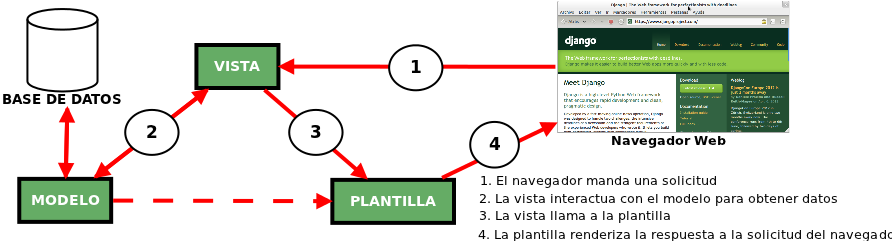
\includegraphics[scale=0.4]{img/esquema-mtv.png}
\end{figure}


\ La arquitectura se divide en cinco bloques:

\begin{itemize}
\item\textbf{settings.py: }aquí se encuentran todas las configuraciones que podemos agregar o modificar para nuestro proyecto, aplicaciones instaladas, Base de datos que va a ser utilizada, directorio de plantillas...
\item\textbf{manage.py }Es un archivo generado automáticamente que sirve para interactuar desde la consola con el proyecto, usando los comandos que podemos ver en la documentación\footnote{\url{https://docs.djangoproject.com/es/1.9/ref/django-admin/}}.
\item\textbf{models.py: }Cada aplicación que se crea tiene su propio models.py. Aunque es posible utilizar Django sin una base de datos, Django cuenta con este mapeador Objeto-Relacional en el que es posible definir la estructura de la Base de datos utilizando código Python. En Django anterior a la versión 1.9, utilizando el comando syncdb se aplicaba la sentencia ``CREATE TABLE'' automáticamente, verificando si las tablas ya existían, y creándolas en caso negativo. En la última versión de Django (1.9) se debe ejecutar el comando ``makemigrations'' y posteriormente ``migrate''.
\item\textbf{views.py: }Archivo que contiene el código que se ejecuta cuando es llamado por una URL. Esta llamada ejecuta la función en el servidor, para preparar la respuesta al cliente en forma de respuesta HTML, template, JSON...  
\item\textbf{urls.py: }Es el archivo que relaciona las URLs del proyecto creado, con las funciones creadas en el archivo ``views.py''. Utiliza expresiones regulares.

\end{itemize}

La salud actual y futura de Django es muy buena, pues ahora está siendo utilizado en aplicaciones tan de moda como son Disqus, Instagram o Pinterest, además de usarse ya en sitios más consolidados como son Mozilla y OpenStack.\\

\subsection{Python} 
\begin{figure}[hbtp]
\centering

\includegraphics[scale=0.1]{img/Python-logo.png} 
\end{figure}
Python es un lenguaje de programación de muy alto nivel, multiparadigma, con el que se puede desarrollar cualquier programa, desde programas para servidores, hasta páginas web. Es un lenguaje interpretado. Este tipo de lenguajes tienen la ventaja de ser independientes de la máquina y del sistema operativo que los ejecute, puesto que no tiene instrucciones propias del procesador. No tiene que compilarse, por lo que resulta más rápido para desarrollarlo y resolver inconvenientes, por contra, su principal desventaja es la velocidad, es algo que debemos tener muy en cuenta a la hora de seleccionar el lenguaje que vamos a utilizar (En nuestro caso, la velocidad de la aplicación no es algo determinante).
Decíamos al principio que es un lenguaje multiparadigma, debido a que soporta programación imperativa, programación funcional, y como no, orientación a objetos. Esto ofrece mucha libertad a los programadores.
Tiene una sintaxis limpia y hace que sea fácilmente legible. En los últimos años se ha popularizado por las siguientes razones:
\begin{itemize}
\item Ofrece gran cantidad de librerías que contienen tipos de datos, y funciones incorporadas en el lenguaje que favorecen la realización de muchas tareas sin necesidad de empezar de cero.
\item Sencillez y velocidad al crear programas. Por norma, los programas en python tienen menos lineas que sus equivalentes en C o Java.
\item Cantidad de plataformas en las que se puede desarrollar, Windows, Mac, Unix...
\item Se puede obtener de manera gratuita  y se puede utilizar con fines comerciales.
\end{itemize}

Es un lenguaje apropiado para empezar a en el mundo del desarrollador, pese a que tiene una sintaxis muy estricta.

\subsection{API de GitHub}
\begin{figure}[hbtp]
\centering

\includegraphics[scale=0.2]{img/githublogo.jpg} 
\end{figure}

GitHub es una plataforma de desarrollo colaborativo para alojar proyectos utilizando el sistema de control de versiones Git.
En este proyecto, he utilizado la API (Application Programming Interfaces) de GitHub para conocer los Forks que tenía un repositorio y también para conocer la fecha de la última actualización.
\begin{lstlisting}[frame=single]
GET /repos/:owner/:repo/forks
\end{lstlisting}


\subsection{Pylint}

Pylint es un programa de código abierto\footnote{\url{https://github.com/PyCQA/pylint}} que analiza código Python. Nos ofrece información sobre cómo está escrito el código analizado, según las normas de estilo PEP-8, y clasifica los errores en 5 tipos, a saber:
\begin{itemize}
\item Refactorización: Asociado a alguna violación en alguna buena práctica.
\item Convención: Asociado a una violación del estándar de codificación.
\item Advertencia: Asociado a problemas de estilo o errores menores en la programación.
\item Error: Son errores importantes en el código, que deben revisarse.
\item Fatal: Si se produce este error, Pylint no pudo terminar el análisis.
\end{itemize}
Pylint es una herramienta que todo programador de python debe considerar para tener un código de buena calidad. Ya que pylint revisa:
\begin{itemize}
\item Presencia de Docstring.
\item Nombres de módulos, clases, funciones, métodos, variables...
\item Uso de declaraciones globales
\item Redefinición de funciones, métodos...
\item Revisión de si las variables son usadas o no
\item Revisión de diseño, e imports
\end{itemize}
Como Pylint es totalmente configurable, se pueden filtrar errores que no queremos que tenga en cuenta.
Al final del análisis, Pylint nos ofrece una puntuación de dicho código.

\subsection{SQLite3}
\begin{figure}[hbtp]
\centering

\includegraphics[scale=0.8]{img/sqlite3.jpg} 
\end{figure}

SQLite es un sistema de gestión de Bases de datos relacional, compatible con ACID (Atomicidad, Consistencia, Aislamiento, Durabilidad), escrita en C. Es de dominio público. \\
A diferencia de los sistema de gestión de bases de datos cliente-servidor, el motor de SQLite no es un proceso independiente con el que el programa principal se comunica. En lugar de eso, la biblioteca SQLite se enlaza con el programa, pasando a ser parte integral del mismo. El programa utiliza la funcionalidad de SQLite a través de llamadas simples a subrutinas y funciones. Esto reduce la latencia en el acceso a la base de datos, debido a que las llamadas a funciones son más eficientes que la comunicación entre procesos. El conjunto de la base de datos (definiciones, tablas, índices, y los propios datos), son guardados como un único fichero estándar en la máquina host. Este diseño simple se logra bloqueando todo el fichero de base de datos al principio de cada transacción.

En su versión 3, SQLite permite bases de datos de hasta 2 Terabytes de tamaño, y también permite la inclusión de campos tipo BLOB (Binary large object).

\section{Tecnologías Cliente} 
\label{sec:seccion2}
\subsection{HTML5} 
\begin{figure}[hbtp]
\centering

\includegraphics[scale=0.3]{img/HTML5.png} 
\end{figure}
Es la última versión de HTML (HyperText Markup Language). El término representa dos conceptos diferentes:
\begin{itemize}
\item Se trata de una nueva versión de HTML, con nuevos atributos, elementos y comportamientos.
\item Cuenta con más tecnologías que permiten a las aplicaciones Web y sitios Web, ser más diversos. A este conjunto se le llama ``HTML5 y amigos'', comunmente HTML5.
\end{itemize}

Esta es la primera vez que se desarrollan en paralelo HTML y XHTML. La versión definitiva se publicó en Octubre de 2014. Las tecnologías de HTML5, se clasifican en varios grupos según su función:
\begin{itemize}
\item \textbf{Semántica: }Describe con más precisión cual es su contenido, añadiendo nuevas etiquetas.
\item \textbf{Conectividad: }Permite comunicaciones con el servidor usando: Web Sockets, Eventos de servidor enviados, WebRTC.
\item \textbf{Sin Conexión y almacenamiento: }Permite a las páginas web almacenar datos localmente en el lado del cliente y operar sin conexión de manera más eficiente
\item \textbf{Multimedia: } Ofrece un excelente soporte para utilizar contenido multimedia, como son audio y vídeo nativamente.
\item \textbf{Rendimiento e integración: }Proporciona una optimización de la velocidad y un mejor uso del hardware
\item \textbf{Acceso al dispositivo: }Proporciona APIs para el uso de varios componentes internos de entrada y salida de nuestro dispositivo (cámara, micrófono, geolocalización...)
\item \textbf{CSS3: }Nueva variedad de opciones para diseños más complejos.
\end{itemize}

\subsection{JavaScript}
\begin{figure}[hbtp]
\centering

\includegraphics[scale=0.85]{img/js.png} 
\end{figure}
A principios de los años 90, la mayoría de usuarios que se conectaban a Internet lo hacían con módems a una velocidad máxima de 28.8 kbps. En esa época, empezaban a desarrollarse las primeras aplicaciones web y por tanto, las páginas web comenzaban a incluir formularios complejos.

Con unas aplicaciones web cada vez más complejas y una velocidad de navegación tan lenta, surgió la necesidad de un lenguaje de programación que se ejecutara en el navegador del usuario. De esta forma, si el usuario no rellenaba correctamente un formulario, no se le hacía esperar mucho tiempo hasta que el servidor volviera a mostrar el formulario indicando los errores existentes.

JavaScript es un lenguaje de programación que se utiliza principalmente para crear páginas web dinámicas.

Una página web dinámica es aquella que incorpora efectos como texto que aparece y desaparece, animaciones, acciones que se activan al pulsar botones y ventanas con mensajes de aviso al usuario.

Técnicamente, JavaScript es un lenguaje de programación interpretado, por lo que no es necesario compilar los programas para ejecutarlos. En otras palabras, los programas escritos con JavaScript se pueden probar directamente en cualquier navegador sin necesidad de procesos intermedios.

A pesar de su nombre, JavaScript no guarda ninguna relación directa con el lenguaje de programación Java. Legalmente, JavaScript es una marca registrada de la empresa Sun Microsystems.

Las \textbf{ventajas }que tiene JavaScript son:
\begin{itemize}
\item Excelente solución para poner en práctica la validación de datos de un formulario en el lado del cliente. Si un usuario omite escribir su nombre en un formulario, una función de validación en JavaScript puede desplegar en pantalla un mensaje popup para hacerle saber al usuario acerca de la omisión.

\item Creación de efectos dinámicos tales como imágenes dinámicas y presentaciones de diapositivas, donde su uso se ha convertido algo común hoy en día.
\end{itemize}
Por contra, sus \textbf{desventajas } son:
\begin{itemize}
\item La seguridad. Los fragmentos de código de JavaScript son descargados y se ejecutan en el navegador del cliente, esto puede provocar que un código malicioso pueda ser ejecutado en la máquina del cliente con el objetivo de explotar alguna vulnerabilidad de seguridad conocida en una de las aplicaciones, navegadores o el mismo sistema operativo.

\item Introduce una gran cantidad de fragmentos de código en los sitios web. El problema es sobretodo  para los motores de búsqueda como, por ejemplo, Google. Este código, hace que sea más complicado descifrar la calidad del contenido, y pueda indexarse correctamente. Por suerte, el problema de grandes fragmentos de código JavaScript se resuelve fácilmente mediante el almacenamiento del código JavaScript dentro de archivos separados del código HTML con la extensión. *.Js, dejando una página web mucho más limpia y legible de cara al desarrollador. 
\end{itemize}

\subsection{CSS3}
\begin{figure}[hbtp]
\centering

\includegraphics[scale=0.35]{img/CSS3.png} 
\end{figure}

Las hojas de estilo llegaron después del lenguaje de etiquetas SGML,cerca del año 1970. Desde la creación de SGML, se observó la necesidad de definir un mecanismo que permitiera aplicar de forma consistente diferentes estilos a los documentos electrónicos.

El gran impulso de los lenguajes de hojas de estilo se produjo con la llegada de Internet y el crecimiento exponencial del lenguaje HTML para la creación de documentos electrónicos. La guerra de navegadores y la falta de un estándar para la definición de los estilos dificultaban la creación de documentos con la misma apariencia en diferentes navegadores. Finalmente el organismo W3C, encargado de definir los estándares relacionados con la web, aceptaron una propuesta que llamaron CSS (Cascading Style Sheets).

En resumen, CSS3 es una tecnología que nos permite crear páginas web de una manera más exacta, y podemos hacer cosas que no podríamos hacer sólo con HTML, como incluir márgenes, tipos de letra, fondos, colores...
\\
\subsection{Bootstrap}
\begin{figure}[hbtp]
\centering

\includegraphics[scale=0.2]{img/bootstrap.png} 
\end{figure}

Bootstrap fue desarrollado por Mark Otto y Jacbod Thornton de Twitter, como un marco de trabajo (framework) para fomentar la consistencia a través de herramientas internas. Antes de Bootstrap, se usaban varias librerías para el desarrollo de interfaces de usuario, las cuales guiaban a inconsistencias y a una carga de trabajo alta en su mantenimiento.

Es un framework de Código abierto para diseño de sitios y aplicaciones web. Contiene plantillas de diseño con tipografía, formularios, botones, cuadros, menús de navegación y otros elementos de diseño basado en HTML y CSS, así como, extensiones de JavaScript opcionales adicionales.

Es uno de los proyectos más populares de GitHub.\footnote{\url{http://web.archive.org/web/20100419140506/http://github.com/popular/watched}} \\
 \textbf{Características:} \
\begin{itemize}
\item Compatible con la mayoría de navegadores web.
\item Diseños sensibles, esto es, que el diseño gráfico de la pantalla se ajusta dinámicamente,tomando en cuenta las características del dispositivo usado.
\item Es de código abierto y disponible en GitHub.
\item Gran apoyo de la comunidad de desarrolladores
\item Sencillez y fácil de implementar
\item Buenos resultados en poco tiempo
\end{itemize}

\textbf{Estructura y funciones: }\
\begin{itemize}
\item Sistema de cuadrilla y diseño sensible.
\item Componentes re-usables.
\item Conjunto de hojas de estilo que proveen definiciones básicas de estilo para todos los componentes de HTML, dando así uniformidad al navegador y al sistema de anchura.
\item Los componentes de JavaScript para Bootstrap están basados en la librería jQuery de JavaScript.
\end{itemize}


%%%%%%%%%%%%%%%%%%%%%%%%%%%%%%%%%%%%%%%%%%%%%%%%%%%%%%%%%%%%%%%%%%%%%%%%%%%%%%%%
%%%%%%%%%%%%%%%%%%%%%%%%%%%%%%%%%%%%%%%%%%%%%%%%%%%%%%%%%%%%%%%%%%%%%%%%%%%%%%%%
% DISEÑO E IMPLEMENTACIÓN %
%%%%%%%%%%%%%%%%%%%%%%%%%%%%%%%%%%%%%%%%%%%%%%%%%%%%%%%%%%%%%%%%%%%%%%%%%%%%%%%%

\cleardoublepage
\chapter{Diseño e implementación}
\section{Arquitectura de la aplicación: } 
La arquitectura para el correcto funcionamiento de la aplicación se basa en la interacción de las tecnologías expuestas en el capitulo 3. \\
En la siguiente imagen, de elaboración propia, están las tecnologías principales para el correcto funcionamiento de la aplicación.
\begin{figure}[hbtp]
\centering
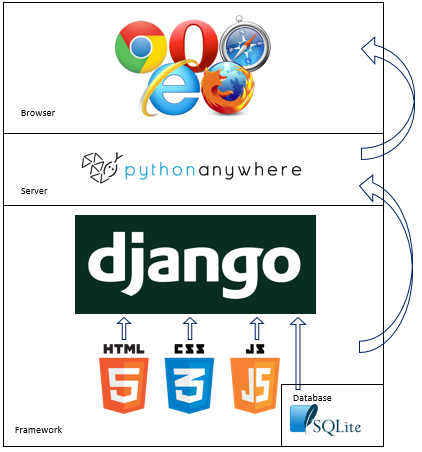
\includegraphics[scale=0.8]{img/arquitectura.png} 
\end{figure}

El navegador es alimentado por el servidor pythonanywhere. Y dentro de pythonanywhere es donde tenemos nuestros ficheros de configuración de Django, con los archivos explicados en el capitulo 3. También, se alojan en pythonanywhere, los archivos HTML, CSS3, y JS que necesita Django.

\section{Base de datos SQLite3: } 

\begin{figure}[H]
\centering
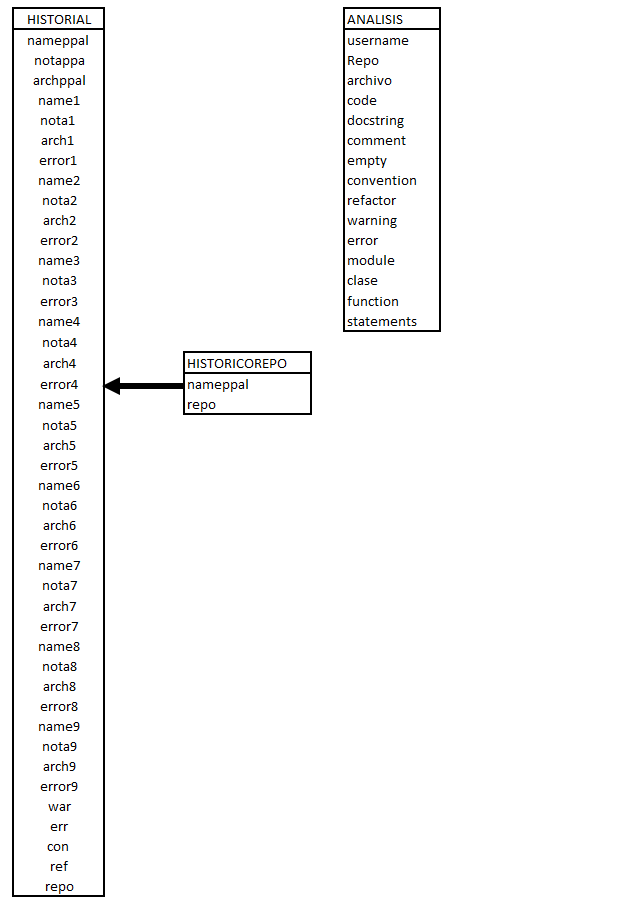
\includegraphics[scale=0.6]{img/tablasBBDD.png} 
\caption{Diagrama con las tablas de la Base de Datos}
\end{figure}
\begin{itemize}
\item \textbf{HistoricoRepo: }En esta tabla guardamos todos los nombres de repositorios que hemos analizado anteriormente, y después hacemos una consulta para poder añadirlos en la columna "historial" del HTML.
\item \textbf{Historial: } Este objeto lo utilizamos para guardar toda la información que mostramos al usuario cuando consulta un análisis. Para que de esta forma sea rápido mostrar sus resultados.
\item \textbf{Análisis: } En este objeto guardamos la información de los errores de un repositorio completo. Sumando los errores de cada archivo, al tipo de error correspondiente. Así podemos analizar los datos rápidamente.

\end{itemize}

\section{Instalaciones necesarias: } 
Todo lo instalado ha sido sobre una distribución de Linux, en mi caso, Ubuntu 15.10.
\subsection{Django}
Para empezar con el proyecto, lo primero que hice fue instalar Django en mi ordenador, para ello ejecuté en un terminal la sentencia: \\
\lstset{language=bash, breaklines=true, basicstyle=\footnotesize}
\begin{lstlisting}[frame=single]
~$ pip install django==1.9
\end{lstlisting}
Una vez acabada la instalación, ya estamos listos para crear un proyecto Django.

\subsection{Pylint}
Pylint es otro programa que tuve que instalar en mi ordenador.
Previamente comprobé qué versión de python estaba usando, puesto que Pylint requiere al menos la versión 2.7 para poder funcionar. Para ello, ejecuté en un terminal la sentencia:\\
\lstset{language=bash, breaklines=true, basicstyle=\footnotesize}
\begin{lstlisting}[frame=single]
~$ python -V
\end{lstlisting}
\newpage
Una vez comprobamos que tenemos una versión de Python, superior o igual a Python 2.7, instalamos Pylint, ejecutando en un terminal la siguiente sentencia:\\
\lstset{language=bash, breaklines=true, basicstyle=\footnotesize}
\begin{lstlisting}[frame=single]
~$ sudo apt-get install pylint
\end{lstlisting}

\section{Nuevo Proyecto: }

Una vez que tenemos el equipo listo, empezamos a crear el proyecto Bestfork.
Creamos un proyecto en Django, ejecutando en un terminal, la sentencia (situándonos en el directorio donde queramos crear el proyecto):\\
\lstset{language=bash, breaklines=true, basicstyle=\footnotesize}
\begin{lstlisting}[frame=single]
~$ django-admin startproject mysite .
\end{lstlisting}

Ahora, tendremos la siguiente estructura:

\begin{figure}[hbtp]
\centering
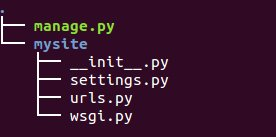
\includegraphics[scale=0.8]{img/tree.jpg} 
\end{figure}

Ahora, que tenemos los archivos necesarios, creamos la aplicación, escribiendo en un terminal:
\lstset{language=bash, breaklines=true, basicstyle=\footnotesize}
\begin{lstlisting}[frame=single]
~/Name$ python manage.py startapp "APPNAME"
\end{lstlisting}   
y conseguimos esta estructura:

\begin{figure}[H]
\centering
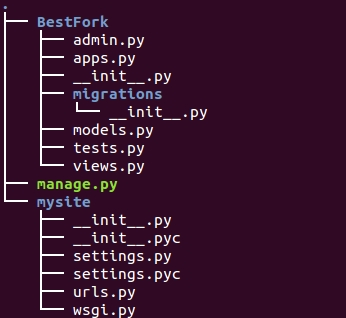
\includegraphics[scale=0.5]{img/treeBig.jpg} 
\end{figure}

Es en el archivo views.py, donde vamos a escribir el código que deseamos que se ejecute en cada URL. Para eso, configuramos el archivo urls.py.

\newpage
\subsection{Esquema del funcionamiento de la aplicación}
\begin{figure}[H]
\centering
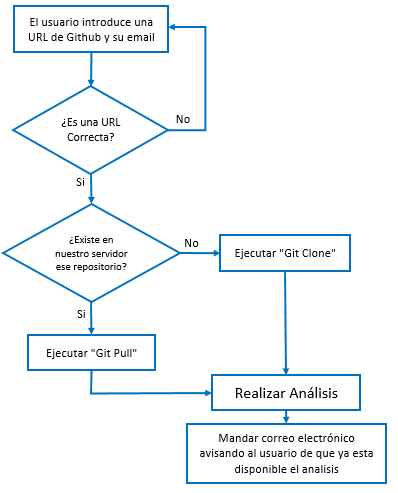
\includegraphics[scale=0.9]{img/DiagramaFlujoTFG1.png} 
\caption{Diagrama de flujo del funcionamiento de la aplicación}
\end{figure}

En este Diagrama de Flujo explico el funcionamiento de la aplicación. 
El usuario introduce una dirección del repositorio en el que esta interesado y su correo electrónico. Si la dirección del repositorio en GitHub no es correcta (se comprueba haciendo uso de la tecnología JavaScript), o la dirección de correo electrónico no tiene formato de correo electrónico, le aparecerá un mensaje indicativo de qué campo no es correcto para que el usuario repita la acción indicando correctamente esos campos.\\
Una vez el usuario ha introducido correctamente esos datos, pasamos a comprobar si tenemos información acerca del repositorio por el que el usuario se interesa. En caso de que ya exista en el servidor, ejecutaremos ``Git Pull'' para tener en cuenta posibles actualizaciones que se hayan producido, en caso contrario, ejecutaremos ``Git Clone'' para descargar ese repositorio. Hay que aclarar que, antes de descargar cualquier repositorio, comprobaremos la última fecha de actualización, quedando fuera de las descargas/actualizaciones todos los repositorios que lleven sin actualizarse más de 180 días. Puesto que la mayoría de repositorios que no sufren cambios en más de ese periodo de tiempo, no vuelven a actualizarse\\
Después de descargar/actualizar los datos necesarios, procedemos al analisis usando Pylint.\\
Cuando el análisis de todos los repositorios ha acabado, enviamos un email al usuario con la url donde puede ver el resultado del análisis rápidamente
\subsection{Página de inicio}
\begin{figure}[H]
 \centering
  \subfloat[Ordenador]{
   \label{f:Ordenador}
    
\includegraphics[width=0.62\textwidth]{img/ppalOrdenador.jpg}}
  \subfloat[Movil]{
   \label{f:Movil}
    
\includegraphics[width=0.22\textwidth]{img/ppalMovil.png}}
 \caption{Vistas}
 \label{f:Vistas}
\end{figure}

Hemos elegido una página principal sencilla, y elegante. \\
La página principal hace dos preguntas que el usuario debe contestar con los datos solicitados.\\
En caso de que la información no se complete, o no se complete correctamente, aparecerá un error, volviendo a solicitar los datos necesarios. Pedimos al usuario un email de contacto, puesto que el análisis se puede demorar bastante, en función del tamaño de este.\\
\begin{figure}[H]
\centering
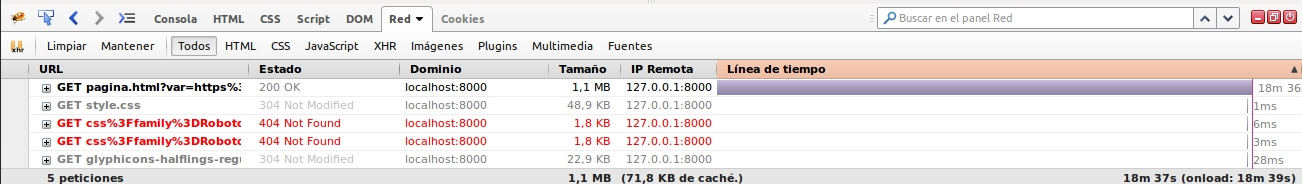
\includegraphics[scale=0.35]{img/tiempo.jpg} 
\caption{Tiempo en analizar un repositorio}
\end{figure}

En el ejemplo, analiza un repositorio con 36 Forks. Cada Fork tiene de media 113 archivos para analizar. El tiempo en nuestra aplicación no lo considero de vital importancia, puesto que el usuario puede introducir el email, y hacer otras cosas hasta que reciba el correo avisándole de que ya está disponible el análisis.

Podemos comprobar en la imagen 4.1, que la página se adapta perfectamente a pantallas más pequeñas como la de un smartphone. Aunque creemos que la mayoría de usuarios que utilicen la aplicación será desde el ordenador, es importante poder verla correctamente desde otro dispositivo.\\ Esto es relevante, puesto que es una de las mayores revoluciones de los últimos años, los smartphones en España ya ocupan más del 54\% de los bosillos\footnote{\url{http://www.abc.es/tecnologia/moviles-telefonia/20140725/abci-ventas-smartphones-tableta-espana-201407251123.html}} y en el planeta ya hay un smartphone por cada cuatro personas. Este dispositivo es lo más cerca que vamos a estar de nuestros usuarios, no hay otro dispositivo que sea tan personal,e inseparable. Si además tenemos en cuenta que en el caso de España y de otros países, el móvil supera al ordenador para acceder a internet, entendemos más aún la necesidad de que la aplicación esté adaptada a Smartphones. Para que estas páginas sean cómodas de usar a través del móvil y tablet, deben tener menús fáciles y cómodos de desplegar, y que sea ligera, puesto que el usuario tiene limitados los datos que puede descargar. En resumen, las páginas han de ser ``responsivas''.

\subsection{Página con el resultado}

\begin{figure}[H]
 \centering
  \subfloat[Ordenador]{
   \label{f:Ordenador}
    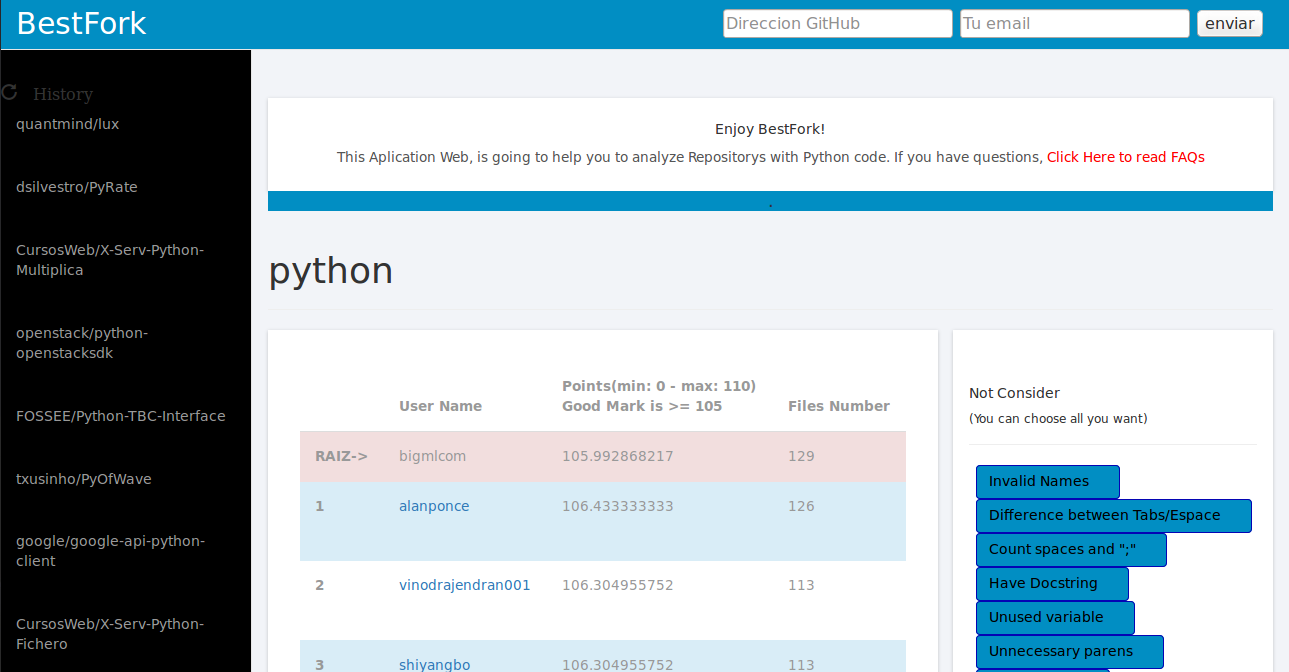
\includegraphics[width=0.62\textwidth]{img/analisislOrdena.png}}
  \subfloat[Movil]{
   \label{f:Movil}
    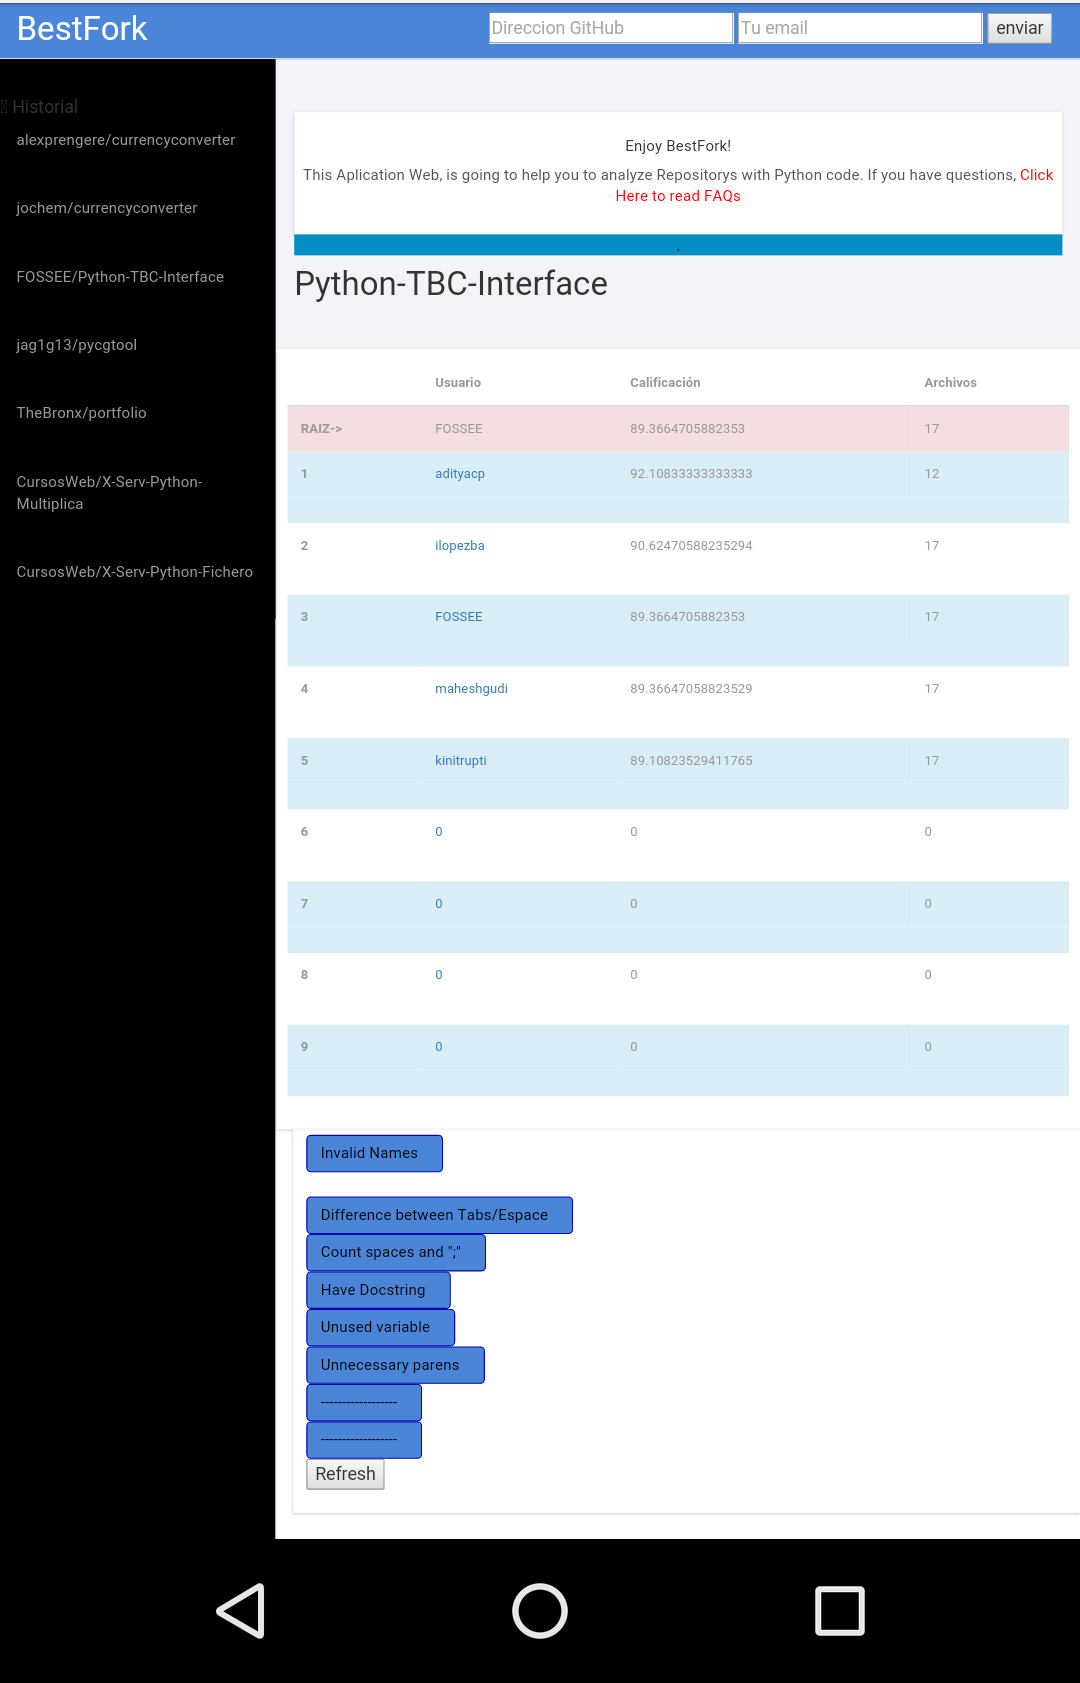
\includegraphics[width=0.22\textwidth]{img/analisislMovil.png}}
 \caption{Vistas}
 \label{f:Vistas}
\end{figure}

La página en la que aparece el análisis es también sencilla. Debía ser una página clara, nada de menús llenos de opciones, una página intuitiva y cómoda, de forma que el usuario entre en la web y en un ``golpe de vista'' entienda lo que mostramos. Por eso esta claramente dividida en 4 zonas, claramente diferenciadas, y es igualmente compatible con teléfonos móviles. 

Analizamos cada zona de la página:

\begin{figure}[hbtp]
\centering

\includegraphics[scale=0.35]{img/barrsuperior.png} 
\caption{Zona Superior}
\end{figure}

Aquí, vemos la zona superior de la página. Con el nombre de la aplicación, y de nuevo, dos cajas para hacer un análisis de otro repositorio que pudiera interesar al usuario. 

\begin{figure}[H]
\centering
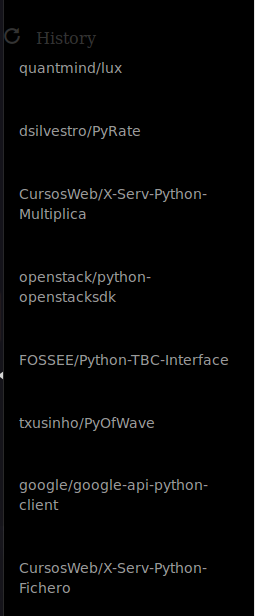
\includegraphics[scale=0.35]{img/barrizq.png} 
\caption{Zona izquierda: Historial}
\end{figure}

En el lado izquierdo de la página, tenemos una columna con el historial de análisis que otros usuarios, o él mismo, han solicitado. Tiene un acceso prácticamente instantáneo, como observamos en la siguiente imagen.

\begin{figure}[H]
\centering
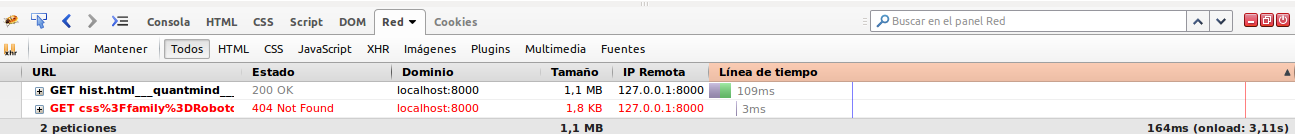
\includegraphics[scale=0.35]{img/tiempoHist.png} 
\caption{Tiempo en ver una página del historial}
\end{figure}

Es un acceso rápido, porque guardamos otros análisis (siempre sin ningún filtro aplicado), en una base de datos y luego solo hace una consulta a esa base de datos.

\begin{figure}[H]
\centering
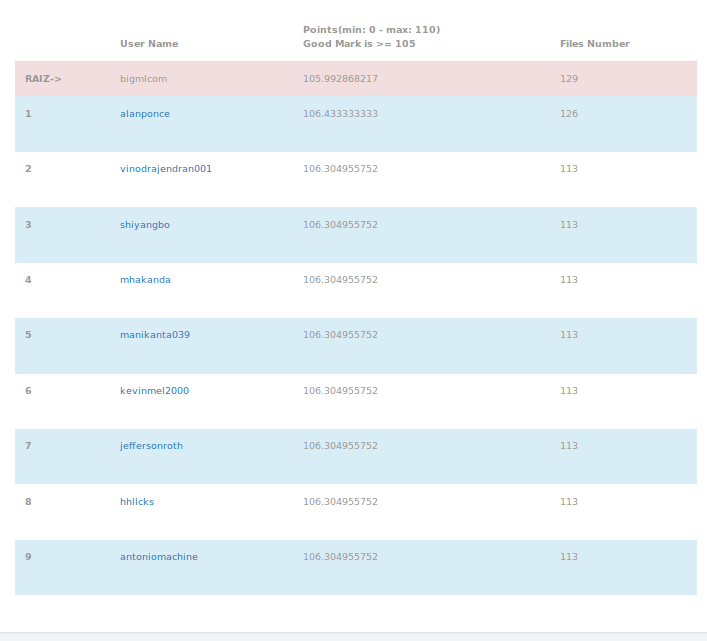
\includegraphics[scale=0.35]{img/medioana.png} 
\caption{Tabla principal}
\end{figure}

Esta tabla, situada en el centro de la página es donde el usuario puede visualizar los resultados obtenidos. El programa Pylint devuelve resultados entre 0-10. Nuestra puntuación va de 0 hasta 110. ¿Por qué? Porque es habitual que en programas de gran tamaño, se acumulen una gran cantidad de fallos y Pylint devuelva una nota negativa\footnote{\url{https://docs.pylint.org/faq.html}}. 

Aún así, recordamos a los usuarios, que una buena nota es cuando el resultado es mayor que 105.\\
Fácilmente, podemos comparar los Forks, con el repositorio principal, que se muestra el primero en una fila roja.\\
Si pulsamos sobre el nombre de alguno de los Forks, nos despliega todos los errores que tiene el código en cada archivo y si volvemos a pulsar, los oculta.
También mostramos el número de archivos que tiene cada Fork.
\newpage
\begin{figure}[H]
\centering
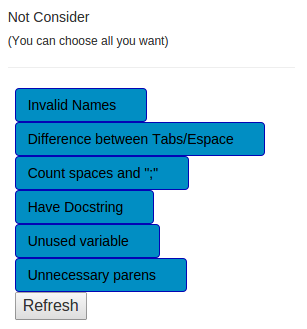
\includegraphics[scale=0.35]{img/filtrosder.png} 
\caption{Parte derecha. Filtros.}
\end{figure}


En esta columna situada a la derecha, el usuario selecciona los filtros que quiere aplicar al análisis para que los resultados se ajusten más a sus necesidades. Los filtros que hemos puesto son los errores que más se repiten en las baterías de pruebas que hemos hecho.\\
Y son los siguientes:
\begin{itemize}
\item Invalid Names: Error cuando un nombre no encaja con la convención de nomenclatura asociada a su tipo
\item Difference between Tabs/Espace: Se utiliza cuando hay espacios y tabulaciones mezclados en una linea
\item Count spaces and ``;'': Se utiliza cuando se usa un número incorrecto de los espacios alrededor de un operador,  o cuando acaba una linea en ``;'' siendo innecesario
\item Have Docstring: Se usa cuando un módulo, la función, la clase o método no tiene ninguna cadena de documentación. Algunos métodos especiales, como init (), no requieren una cadena de documentación, pero esto se tiene en cuenta.
\item Unused variable: Se utiliza cuando se ha declarado una variable, pero no se esta utilizando a lo largo del código.
\item Unnecessary parens: Se utiliza cuando en alguna linea hay más paréntesis de los que realmente se necesitan.
\end{itemize}
Al pulsar en el botón actualizar, se procederá a recalcular la nota de todos los repositorios teniendo en cuenta la selección del usuario. Mientras esto ocurre, se le ocultan los botones al Usuario para que no interfiera con las operaciones que está haciendo el servidor. Además, aparece una animación informando al usuario que se está cargando el análisis.\\
Esto es, sobretodo, para hacer al usuario consciente de que se está cargando su análisis, y no parezca que la página no está respondiendo a su petición, ya que la operación puede demorarse varios minutos, en caso de que fuese un repositorio con muchos Forks, y/o archivos Python.

\begin{figure}[H]
\centering
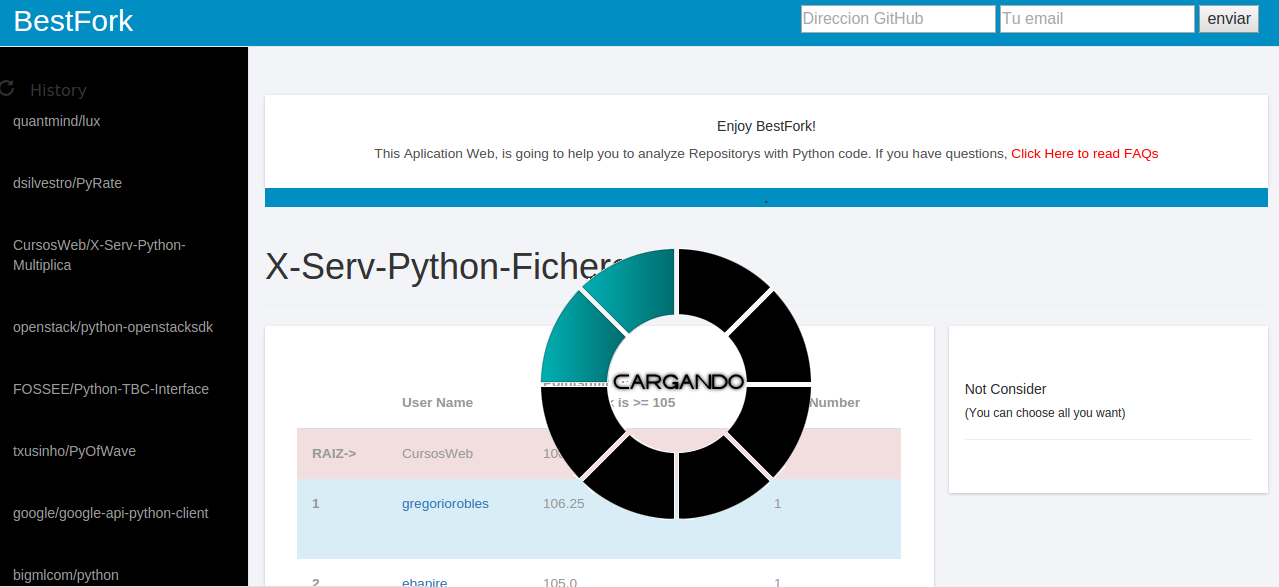
\includegraphics[scale=0.35]{img/charge1.png} 
\caption{Ejemplo de la página actualizando}
\end{figure}
\newpage
\subsection{Página FAQs}
\begin{figure}[H]
\centering
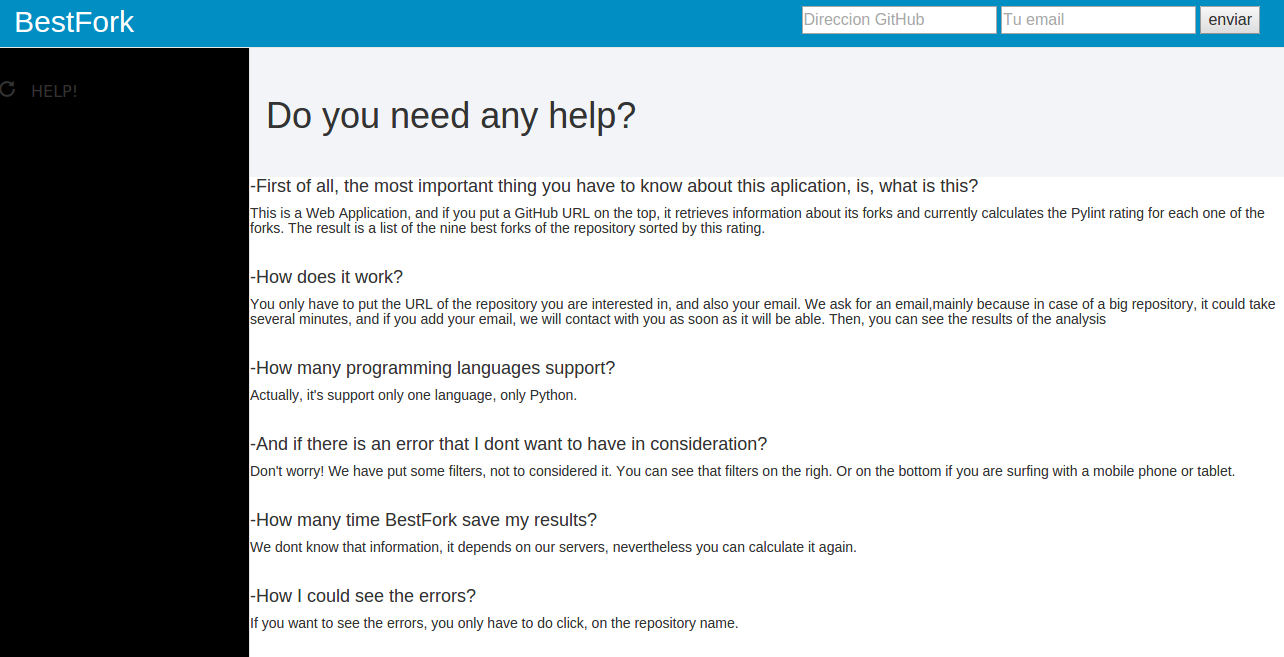
\includegraphics[scale=0.35]{img/faqs1.png} 
\caption{Página de ayuda}
\end{figure}
Pese a que hemos intentado, que la web, sea intuitiva y cómoda, puede que algunos usuarios tengan dudas sobre el funcionamiento de la misma, por eso creamos una página con las posibles preguntas más frecuentes (FAQs).\\
Creemos que cualquier página que tenga alguna interacción con el usuario debe incluir una página donde se respondan las Frequently Asqued Questions, y que sea de acceso rápido, y directo a la información.\\




%%%%%%%%%%%%%%%%%%%%%%%%%%%%%%%%%%%%%%%%%%%%%%%%%%%%%%%%%%%%%%%%%%%%%%%%%%%%%%%%
%%%%%%%%%%%%%%%%%%%%%%%%%%%%%%%%%%%%%%%%%%%%%%%%%%%%%%%%%%%%%%%%%%%%%%%%%%%%%%%%
% RESULTADOS %
%%%%%%%%%%%%%%%%%%%%%%%%%%%%%%%%%%%%%%%%%%%%%%%%%%%%%%%%%%%%%%%%%%%%%%%%%%%%%%%%

\cleardoublepage
\chapter{Resultados}

Para poder conseguir resultados reales, decidimos subir la página a ``pythonanywhere.com'' para que la aplicación tuviera visibilidad desde cualquier lugar. He elegido pythonanywhere.com, porque aunque hacer funcionar Django aquí no fue una tarea trivial, si ofrecían un servicio aceptable en su versión gratuita, y en caso de que en el futuro quisiéramos un mejor servicio, los precios eran los más econónimos comparándolo con hostgator.com o Heroku, que son las alternativas que barajamos.\\
Teniendo el servidor en mi ordenador personal, no tenía ningún problema en cuanto al tamaño del repositorio que quería analizar, puesto que contaba con alta velocidad de conexión a internet, y buena velocidad de CPU para analizar los repositorios, pero al subir la aplicación a Pythonanywhere.com se me presentó el problema de que usando la versión gratuita, tenía limitaciones en lo referente al ancho de banda, al espacio disponible, y la baja velocidad de CPU que me ofrecían.\\
Como los consumos de la aplicación, dependen directamente del repositorio a analizar, para las pruebas utilizaría repositorios de tamaño moderado.

Fui buscando repositorios, con contenido cuyo código estuviese escrito en Python. Encontré un repositorio de un portfolio con varios archivos escritos en Python. El repositorio contaba con 10 archivos, y ningún Fork, por lo que no tendría problema en analizarlo en ``pythonanywhere.com''.\\
Empecé ejecutando en el terminal: 
\begin{lstlisting}[frame=single]
git clone https://github.com/TheBronx/portfolio.git
\end{lstlisting}

De esta forma, tenía exactamente la misma puntuación que el usuario previo en la aplicación BestFork.
Analicé los errores que presentaban sus lineas de código, y trabajé para depurar su código, sobre los errores que arrojaba la aplicación BestFork.\\
Una vez había corregido errores que no afectaban directamente al funcionamiento del su programa, lo analicé de nuevo con la aplicación BestFork, y obtuve unas décimas de mejora.

\begin{figure}[H]
\centering
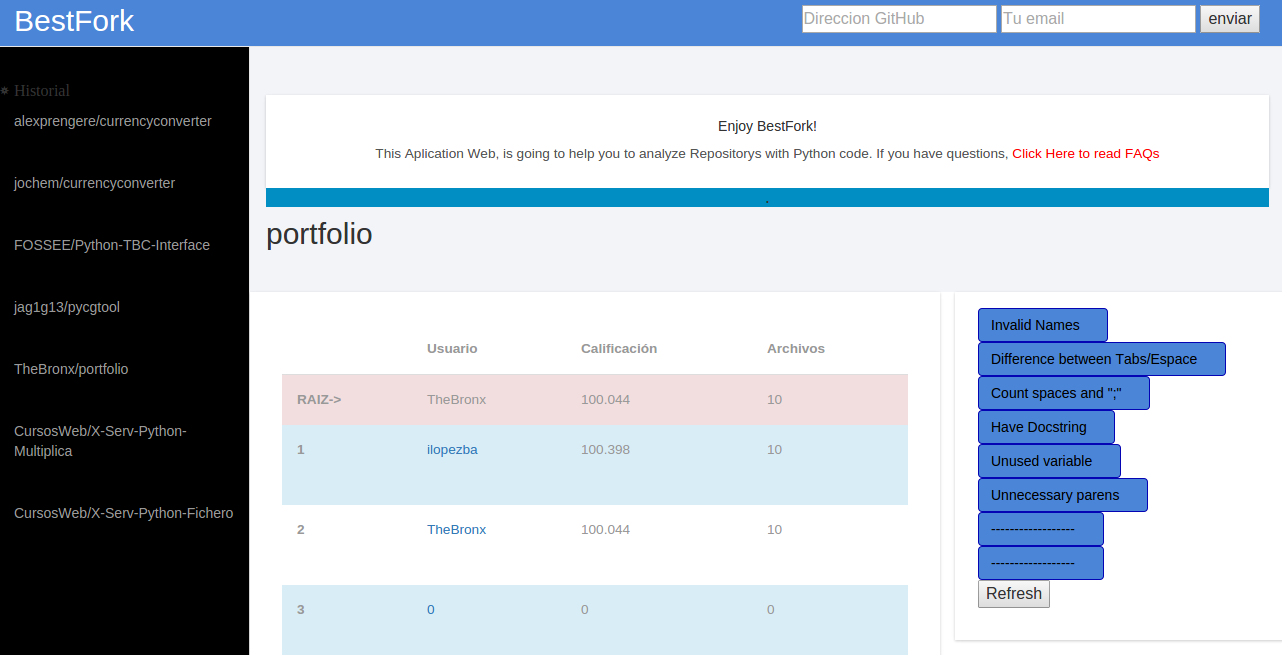
\includegraphics[scale=0.35]{img/mejora.png} 
\caption{Captura de un repositorio con un fork}
\end{figure}

En tan sólo unas horas, había depurado su código y cualquier persona podía comprobar que mi código arrojaba una mayor puntuación que el repositorio principal, gracias a corregir errores. Además, el mismo dueño del repositorio podía comprobarlo en la página web.\\
Con estos datos, creé un Pull Request con la esperanza de que lo aceptase, e hiciese un merge de mi propuesta a su código.

\begin{figure}[H]
\centering
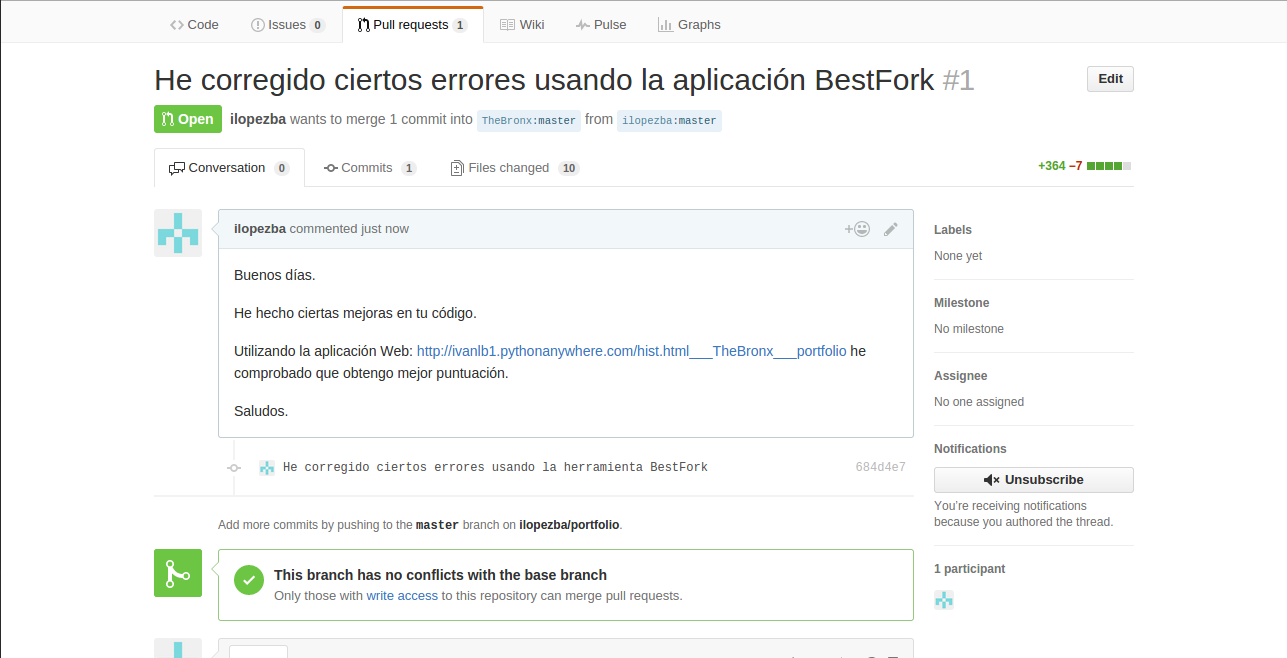
\includegraphics[scale=0.35]{img/pullrequest1.png} 
\caption{Captura de la creación de un pull request}
\end{figure}

Tras mandar el pull request. El usuario dueño del repositorio principal hizo un merge de mi código en su código, aceptando así los cambios que le propuse.
\begin{figure}[H]
\centering
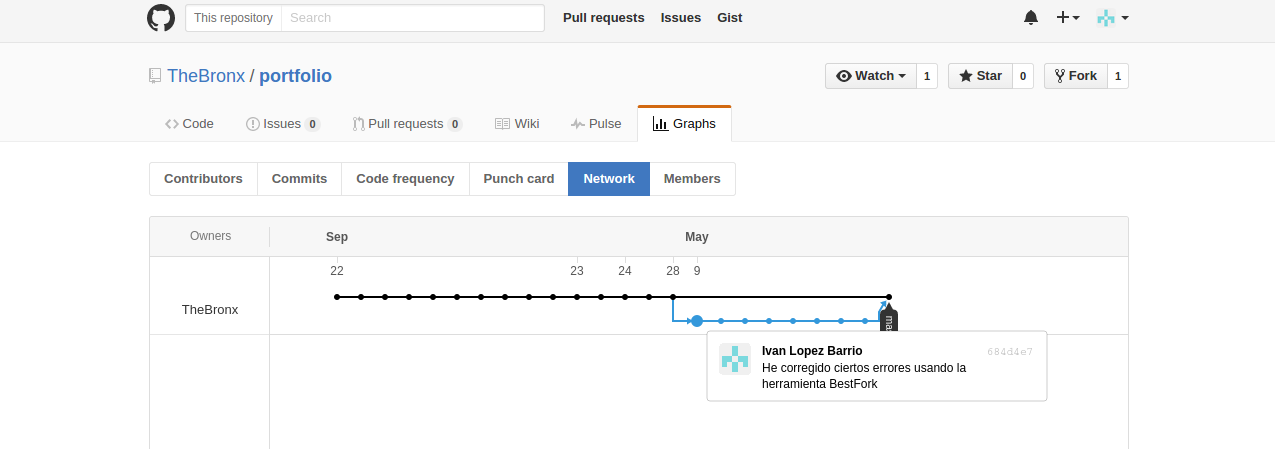
\includegraphics[scale=0.35]{img/merge1.png} 
\caption{El usuario hace merge de mi pull request}
\end{figure}

Tras el merge, le pedimos a la aplicación que nos analice de nuevo el repositorio y sus Forks. El resultado, no es ninguna sorpresa, tanto mi fork, como el repositorio principal obtienen la misma puntuación.
\begin{figure}[H]
\centering
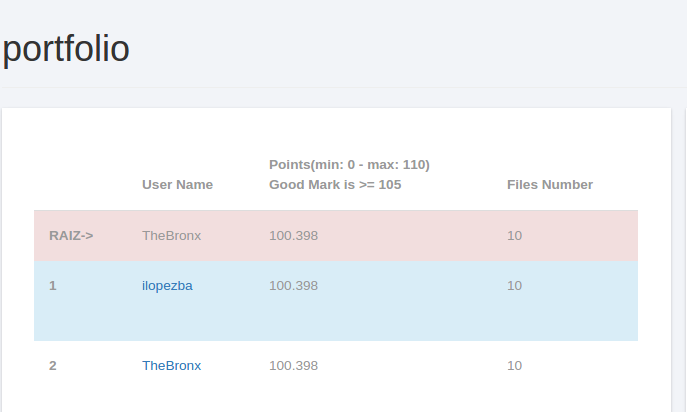
\includegraphics[scale=0.35]{img/puntuacionigual.png} 
\caption{Puntuaciones trás el merge}
\end{figure}
Con esta prueba, queremos demostrar que cumplimos uno de los objetivos específicos, que describimos como: \textbf{ Argumento para crear un Pull Request}, en la memoria de este mismo proyecto.

También, hemos querido demostrar otro de los objetivos específicos, \textbf{Para dueños del repositorio}. Este es un ejemplo de un repositorio educativo, donde la forma de entrega de sus trabajos, es haciendo un Fork de la rama que ofrecen los profesores.\\\

Con esta aplicación, los dueños del repositorio, en este caso, los profesores, pueden ver quienes son, a priori, los alumnos que están llevando a cabo un mejor trabajo. 

\begin{figure}[H]
\centering
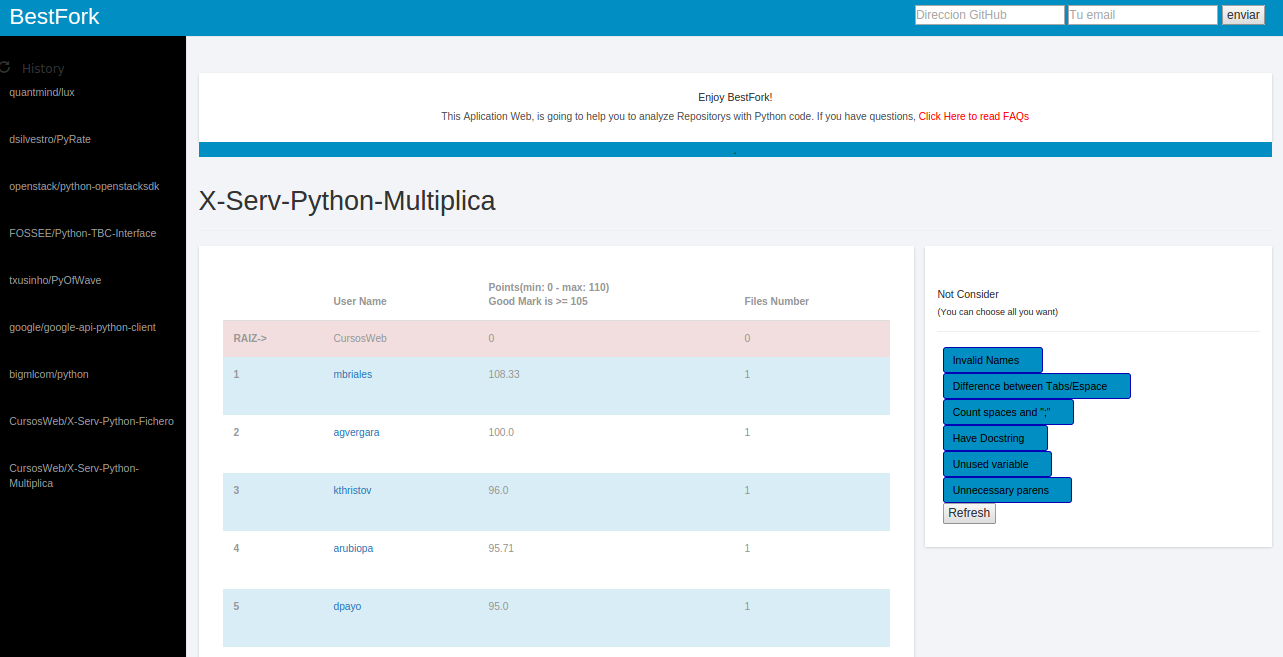
\includegraphics[scale=0.35]{img/puntalumnos.png} 
\caption{Puntuaciones alumnos}
\end{figure}

En tan sólo unos minutos, puedes hacer una breve comparativa de todos los Forks, para ver como evolucionan, en este caso, los alumnos. Además, podemos adelantar fallos comunes que se observen en la mayoría de alumnos para advertirles.\\








%%%%%%%%%%%%%%%%%%%%%%%%%%%%%%%%%%%%%%%%%%%%%%%%%%%%%%%%%%%%%%%%%%%%%%%%%%%%%%%%
%%%%%%%%%%%%%%%%%%%%%%%%%%%%%%%%%%%%%%%%%%%%%%%%%%%%%%%%%%%%%%%%%%%%%%%%%%%%%%%%
% CONCLUSIONES %
%%%%%%%%%%%%%%%%%%%%%%%%%%%%%%%%%%%%%%%%%%%%%%%%%%%%%%%%%%%%%%%%%%%%%%%%%%%%%%%%

\cleardoublepage
\chapter{Conclusiones}
\label{chap:conclusiones}

Como hemos ido viendo a lo largo de la memoria, Bestfork es una aplicación con un potencial realmente elevado. Hemos utilizado las últimas Tecnologías Web que han permitido que el diseño de la página sea sencillo y atractivo. En todo momento he intentado orientar la página hacia la practicidad, una interfaz limpia para que el usuario no tuviese demasiadas cosas en pantalla que le distrajesen del resultado final, evitando en la medida de lo posible que tuviese que hacer scroll para ver los resultados. Que el diseño se vea moderno y sea responsivo, se debe fundamentalmente a Bootstrap, que facilita mucho el trabajo de diseño de la página, y te ofrece herramientas para adaptar la interfaz a otros tamaños de pantalla, algo imprescindible en cualquier aplicación web que se diseñe hoy en día.\\ 
El lenguaje que analizamos ahora mismo es únicamente Python, que es un lenguaje muy utilizado y uno de los más activos en los repositorios de GitHub\footnote{\url{http://www.muylinux.com/2015/08/21/lenguajes-programacion-abiertos-github}}. Era importante elegir un lenguaje con muchos desarrolladores detrás para que empiece a darse a conocer cuanto antes.\\
Al principio del trabajo, me preocupaba el tiempo que tardaba en analizar los repositorios, y ahí surgió la idea de mandar un correo electrónico cuando estuviese listo el análisis.
Respecto a los resultados, estoy realmente satisfecho. Hemos podido demostrar como un desarrollador con bastante actividad dentro de GitHub, y por internet, ha aceptado un pull request de un usuario como el mío, que cuenta con poca trayectoria y poco código dentro de GitHub. Considero que esto ayuda a entender lo fácil que es mejorar el código de un repositorio con BestFork. \\
La aplicación Web, aunque está en inglés, no presentará ninguna dificultad de uso para ninguna persona que no conozca el idioma, puesto que es muy intuitiva.


\section{Consecución de objetivos}
\label{sec:consecucion-objetivos}

Visto lo expuesto a lo largo de la memoria, y apoyándonos en las demostraciones del Capítulo 5 llegamos a la conclusión de que hemos cumplido los objetivos fijados al comienzo de esta memoria.
Hemos querido demostrar, a su vez, que aparte de haber creado una aplicación Web que funciona, es una aplicación útil y que aún tiene un largo camino por delante.

Al comienzo del proyecto, siempre enfocaba el objetivo hacia ``Controlar repositorios propios'' pero según iba desarrollando la aplicación, iba abriendo nuevos horizontes, empezando a ser consciente de que la aplicación tenía muchas más funciones, y por eso ampliamos los objetivos de la aplicación.

\section{Aplicación de lo aprendido}
\label{sec:aplicacion}

Durante mi formación en la Universidad Rey Juan Carlos, he tenido la oportunidad de aprender y formarme en varios campos. He adquirido una serie de habilidades que me han servido para realizar este proyecto más fácilmente. Algunas de estas habilidades son:
\begin{enumerate}
  \item La programación es una de las bases de este proyecto. Cuando empecé la universidad no sabía nada acerca de la programación, y las asignaturas como ``Fundamentos de la programación'', ``Programación de Sistemas de Telecomunicación'' o ``Sistemas Operativos'' entre otras, fueron las que me dieron las bases de programar en practicamente cualquier lenguaje, puesto que conozco las posibilidades que hay en la programación, y ``sólo'' es aprender a escribirlas en otro lenguaje.
  \item También había utilizado Python, lenguaje utilizado en la asignatura ``Laboratorio de Administración y Gestión de Redes y Sistemas'' que ha sido uno de los lenguajes más utilizados en el desarrollo de esta aplicación puesto que en Django los views se escriben en este lenguaje.
  \item Uso de los lenguajes de programación Web (HTML5, Javascript y CSS3), y del framework Bootstrap, conceptos que se impartieron en la asignatura ``Aplicaciones Telemáticas'' y que han hecho que el cliente tenga una mejor experiencia mientras navega por la página web.
  \item Capacidad para aprender de manera autónoma nuevos conocimientos y técnicas adecuados para la concepción, y el desarrollo de nuevas aplicaciones. Esto es algo que no he aprendido en ninguna asignatura en concreto, sino a lo largo de mi vida estudiantil y que en el proyecto he tenido que poner en práctica más que nunca.
  \item Capacidad para entender la API de Github. En las asignaturas relacionadas con Java y Android, aprendí lo que eran las APIs y para qué servían. Cuando me enfrenté a la API de Github, no tuve ningún problema en comprender como utilizarla.
\end{enumerate}


\section{Lecciones aprendidas}
\label{sec:lecciones_aprendidas}
Arrancar con el proyecto fue algo costoso, ya que había tecnologías que nunca había utilizado y, por tanto, tuve que aprenderlas de cero. Aunque esto jugase en mi contra al comienzo, es algo que con el tiempo se volverá a mi favor, puesto que he obtenido conocimientos que me servirán, como por ejemplo:

\begin{enumerate}
  \item Manejo de \LaTeX . Herramienta que he utilizado para redactar esta memoria, a pesar de ser poco intuitiva a primera vista, rápidamente salen a relucir sus ventajas por hacerlo todo bastante más sencillo.
  \item Servidor Django. Nunca había usado esta tecnología para implementar un servidor basada en la arquitectura Modelo-Vista-Controlador. 
  \item Aprendizaje de comandos para configurar el servidor django con la base de datos SQLite3
  \item También, he aprendido a planificar un proyecto. Desde planificar mi auto-formación en Django y SQLite3, hasta la ejecución del proyecto en los plazos establecidos.
  \item Pylint. No sabía de la existencia de programas que evaluaban la calidad de un código de programación. He aprendido qué tipo de errores analizar, a comprender los ficheros que devuelve, y a customizarlo para sacar más partido a sus analisis.
\end{enumerate}

\section{Trabajos futuros}
\label{sec:trabajos_futuros}

Todo el software puede mejorarse. En este caso, es la primera versión de BestFork y su margen de mejora es muy alto.\\
\begin{enumerate}
  \item \textbf{Analizar más lenguajes:} Actualmente, BestFork sólo analiza un lenguaje de programación de entre todos los que hay. Por ello una buena mejora sería que el usuario seleccionase el lenguaje, o mejor aún, poder analizar varios lenguajes de un mismo repositorio. De esta forma, obtendríamos una puntuación del repositorio todavía más fiable y concreta.
  \item \textbf{Analizar en Background:} Muy interesante
   sería que el servidor analizase la petición en segundo plano para que el usuario pueda pedir analizar más repositorios sin esperar a tener los resultados del anterior.
    \item \textbf{Ampliar filtrado:} En mi proyecto, hemos puesto 6 filtros que son los errores más comunes que hemos observado, de todas formas puede que un usuario esté interesado en no tener en cuenta cierto error. Por ello, podían ampliarse, o bien, que el usuario introdujese el número de error de Pylint que no quiere tener en cuenta y así poder customizar mejor el resultado.
  \item \textbf{Analizar errores más repetidos:} Hacer un análisis de los errores más cometidos por los desarrolladores de un repositorio, puede ayudar a filtrar mejor los resultados
    \item \textbf{Mejorar tiempos de análisis:} Aunque, como ya hemos explicado en la memoria, no es algo fundamental que una aplicación sea más rápida, siempre es más interesante. Por ello, creemos que un servidor que use threads al analizar los repositorios (en caso de tener un procesador compatible) mejoraría los tiempos en analizar los repositorios.
        \item \textbf{Seguridad:} Podrían surgir ataques informáticos. Ahora mismo, estamos muy expuestos a sufrir un ataque de denegación de servicio (DDoS).
\end{enumerate}

\section{¿Por qué elegí este proyecto?}
Tenía claro que quería un proyecto que realmente me sirviese para aprender, y quería usar tecnologías relacionadas con la web.\\
Me dirigí al profesor Gregorio, porque me gustó su forma de dar las clases. Además, una asignatura que impartió, iba relacionado con la Web.\\
Al hablar con él, me contó que tenía este proyecto en el que él había trabajado un poco, y me llamó mucho la atención porque iba a aprender Django, iba a trabajar con Python, lenguaje que me gusta, y también iba a usar la API de Github, que me parecía muy interesante.\\
Me motivó bastante el hecho de que considero que es algo que funciona y es realmente útil.\\
Como futuro ingeniero, me gusta hacer cosas que funcionen, y que tengan utilidad.


\section{Valoración personal}
\label{sec:valoracion}

Llegados a este punto, creo que es momento de echar la vista atrás para ver como ha ido evolucionando el proyecto hasta ser lo que es ahora. Repasando todo lo que he ido evolucionando sólo puedo decir que estoy muy satisfecho con el trabajo realizado.\\
En estos meses he compaginado trabajo-TFG-Prácticas. Algunos días he ido al trabajo o a las prácticas, y en la cabeza sólo llevaba el TFG con algún problema que me había surgido, y en esas horas buscaba darle solución. Los mayores problemas venían cuando utilizaba tecnologías que no había practicado nunca, y tenía algún problema. Pero estoy muy contento de ver cómo he ido superando todas las adversidades que iban surgiendo.\\
Creo que he complementado muy bien todo lo aprendido durante la carrera, puesto que he aplicado lo que ya sabía. Además, he aprendido cosas que, estoy seguro, utilizaré algún día en algún otro proyecto real.\\
Con este proyecto, doy por finalizada una muy buena etapa de mi vida, para empezar otra completamente diferente. No sé como será la nueva etapa, pero para la que cierro sólo tengo buenas palabras.



%%%%%%%%%%%%%%%%%%%%%%%%%%%%%%%%%%%%%%%%%%%%%%%%%%%%%%%%%%%%%%%%%%%%%%%%%%%%%%%%
%%%%%%%%%%%%%%%%%%%%%%%%%%%%%%%%%%%%%%%%%%%%%%%%%%%%%%%%%%%%%%%%%%%%%%%%%%%%%%%%
% APÉNDICE(S) %
%%%%%%%%%%%%%%%%%%%%%%%%%%%%%%%%%%%%%%%%%%%%%%%%%%%%%%%%%%%%%%%%%%%%%%%%%%%%%%%%

\cleardoublepage
\appendix
\chapter{Mejora imposible de implementar en Pythonanywhere.com}
\label{app:Trabajo en Background}

Una de las mejoras que propongo, la he intentado implementar para este mismo proyecto. Se trata de analizar los repositorios en background.\\
Me parece una idea interesante, que garantiza una buena experiencia para el usuario con la aplicación.\\
La mejora la tenemos programada y funciona perfectamente en todas las pruebas que hemos realizado localmente pero, por desgracia, el Host (www.pythonanywhere.com), donde decidimos subir la aplicación. Hoy en día tiene deshabilitada la opción de usar threads, tanto en la versión gratuita, como en la versión de pago.
Para realizar esta mejora tuvimos que importar el módulo ``threading'', añadiendo la siguiente línea al principio del código:
\lstset{language=python, breaklines=true, basicstyle=\footnotesize}
\begin{lstlisting}[frame=single]
import threading
\end{lstlisting}

Luego, modificamos la función a la que llamamos al pulsar el botón ``send'', creando un thread que se ocupe de hacer el análisis y añadir todos los datos a la base de datos, con estas líneas:
\lstset{language=python, breaklines=true, basicstyle=\footnotesize}
\begin{lstlisting}[frame=single]
    hMiHilo = NewHilo(response)
    hMiHilo.start()
\end{lstlisting}
\newpage
y ``New Hilo'' es la siguiente clase de python:
\lstset{language=python, breaklines=true, basicstyle=\footnotesize}
\begin{lstlisting}[frame=single]
class NewHilo(threading.Thread):
    def __init__(self, ruta):  
        threading.Thread.__init__(self) 
        self.ruta = ruta 
        self.stoprequest = threading.Event()
    def run(self):
        PrincipalMain(self.ruta)
\end{lstlisting}

Siendo ``PrincipalMain'' la función que va a ejecutar analizando todo lo necesario, y enviando el email al usuario cuando la información esté disponible.

Al modificar el funcionamiento interno de la aplicación, también modificamos la página principal de la aplicación, añadiendo un ``check'' donde el usuario confirmaba que entendía que cuando los datos estén disponibles recibirá un email. De esta forma, informamos al usuario de lo que va a ocurrir cuando pulse el botón ``Send''. Aquí vemos como quedaría el HTML:
\begin{figure}[H]
\centering

\includegraphics[scale=0.35]{img/threadppal.png} 
\caption{Tiempo en analizar un repositorio}
\end{figure}

Al pulsar ``Send'' mandará la información, y en Background empezará a analizar el repositorio, mientras el usuario permancerá en la misma página, pudiendo así introducir una nueva URL para ser analizada.

\section{Esquema del funcionamiento de la aplicación utilizando threads}
\begin{figure}[H]
\centering
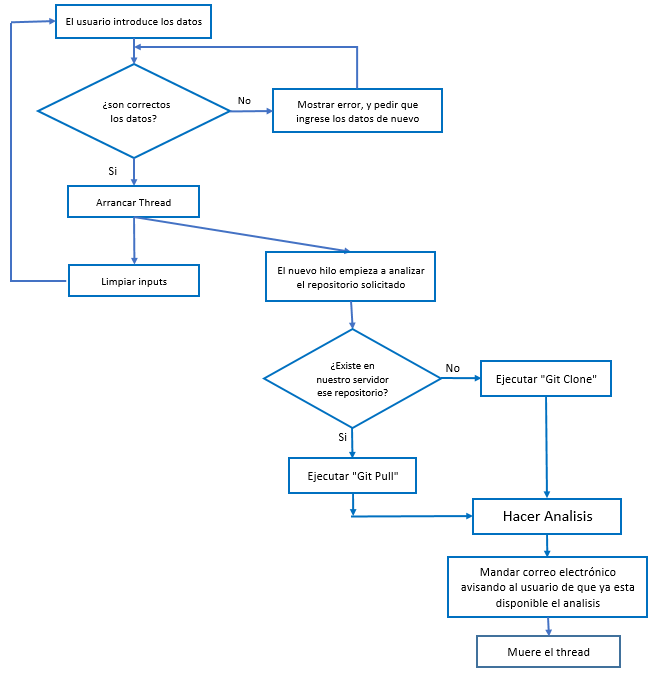
\includegraphics[scale=1]{img/DiagramaThread.png} 
\caption{Esquema con threads}
\end{figure}


%%%%%%%%%%%%%%%%%%%%%%%%%%%%%%%%%%%%%%%%%%%%%%%%%%%%%%%%%%%%%%%%%%%%%%%%%%%%%%%%
%%%%%%%%%%%%%%%%%%%%%%%%%%%%%%%%%%%%%%%%%%%%%%%%%%%%%%%%%%%%%%%%%%%%%%%%%%%%%%%%
% BIBLIOGRAFIA %
%%%%%%%%%%%%%%%%%%%%%%%%%%%%%%%%%%%%%%%%%%%%%%%%%%%%%%%%%%%%%%%%%%%%%%%%%%%%%%%%

\cleardoublepage

% Las siguientes dos instrucciones es todo lo que necesitas
% para incluir las citas en la memoria
\bibliographystyle{abbrv}
\bibliography{memoria}  % mArgumento para crear un "pull request"emoria.bib es el nombre del fichero que contiene
% las referencias bibliográficas. Abre ese fichero y mira el formato que tiene,
% que se conoce como BibTeX. Hay muchos sitios que exportan referencias en
% formato BibTeX. Prueba a buscar en http://scholar.google.com por referencias
% y verás que lo puedes hacer de manera sencilla.
% Más información: 
% http://texblog.org/2014/04/22/using-google-scholar-to-download-bibtex-citations/

\end{document}
